%%
% 下のコメント欄は卒論執筆時の森がイキって書いたものです。
% 修論執筆時の森が代わりに謝罪いたします。
% 温かい目で見守ってあげてください。
%
% また、修論執筆時にはTeXstudioで、またDockerを用いて執筆しています。
% 上記の手法は平木場くんから教えていただきました。
% 参考: https://qiita.com/Shitimi_613/items/9706d57fb7bc17cbed0e
%

%%
% モダンなLaTeXを書きたい?
% そしたら僕の考えた最強のtexファイルを見てくれ
%
% 注意!
% このLaTeXをPDFに変換するためには、普通とはちょっと違う方法を使うよ
% コマンド上では
%   $ ptex2pdf -u -l GraduatePaper.tex
% で変換してね
% もしptex2pdfコマンドが無かったら、
%   $ uplatex GraduatePaper.tex
%   $ dvipdfmx GraduatePaper.dvi
% でうまくいくかも(未確認)
%
% え、TeXworksで使いたいって?
% そしたら、TeXworksの編集メニュー -> 設定を開く
% タイプセットタブの下の方にあるタイプセットの方法の右下の+ボタンを選択する
% 名前: uplatex(ptex2pdf)
% プログラム: ptex2pdf
% 引数: -l
%       -u
%       -ot
%       $synctexoption
%       $fullname
% として保存して、TeXworks実行ボタン右のコンボボックスのuplatex(ptex2pdf)を選択して変換だ!
%


%%
% 今時jarticleやjbook使ってる人いる?時代はjsarticleかjsbookだよ
% ついでに言うと、uplatexってのはplatexの上位互換、これを使わないなんて旧世代だよね
%
\documentclass[uplatex, report, a4j, 10pt, dvipdfmx]{jsbook}


%%
% パッケージ群
%
\usepackage{packages/miyazaki-u-paper}   % 宮崎大学工学部の卒論の基本(片山先生作)を、僕がちょっと書き換えちゃった(テヘッ
\usepackage{enumitem}           % enumerate?古い古い
\usepackage[dvipdfmx]{graphicx, color} % 当然dvipdfmなんて使ってないよね
% \usepackage[dvipdfmx]{color}    % listingsを使うときにはこれも必須、dvipdfmxを変えちゃうとgraphicxのdvipdfmxも変わるよ
\usepackage{listings, packages/jlisting} % コードを埋め込むなら必須
\usepackage{txfonts}            % フォントといえばやっぱりtxfonts、今はnewtxってのもあるらしい
\usepackage{verbatim}           % コメントアウトしてくれる便利なプリアンブルが使える \begin{comment} ... \end{comment}
\usepackage[hdivide={21mm, , 21mm}, vdivide={30mm, , 25mm}]{geometry} % スタイルを少し変えたくても\hoffset, \voffsetは使わないでね
\usepackage[dvipdfmx]{hyperref} % リンクを付けてくれる。
\usepackage{pxjahyper}          % リンクを付けてくれる(日本語)
\usepackage[htt]{hyphenat}      % textttをハイフネーションしてくれる。
%\RequirePackage[l2tabu, orthodox]{nag} % これを入れると、古いコマンドを警告してくれる!なお完全には消せなかった模様

%%
% font周りのwarningを消す。
% https://www.semipol.de/2018/06/12/latex-best-practices.html#filtering-warnings
%
\usepackage{silence}% http://ctan.org/pkg/silence
\WarningFilter{latexfont}{Font shape}
\WarningFilter{latexfont}{Some font shapes}


%
% マクロの定義
%
\newcommand{\tool}{TOOL}
\newcommand{\toolFullName}{TOOL: Optimize Operation Language}

\usepackage{languages}   % 言語設定ファイル

%%
% miyazaki-u-paper.sty用設定値
%
\degree{m} % Graduateのg or Masterのm
\figurenumbering{f} % 図目次を付ける場合はt (真) を持つ真偽値を引数に取る関数
\tablenumbering{f} % 表目次を付ける場合はt (真) を持つ真偽値を引数に取る関数
\title{長ったらしいタイトルを \\ リアルタイムに描画するツール \\ \tool{}の実装と評価}
\author{執筆者ネーム}
\nendo{30} % 年度
\advisor{片山 徹郎 教授} % 修論では無視する
\major{工学専攻 機械・情報系コース 情報システム工学分野}



\begin{document}
\maketitle

\preface{概要}

ここには概要を書くよ


%%
% 本文
%
% はじめに
\chapter{はじめに}\label{cha:Introduction}

ここには初めにをかくほ

以下、本論文の構成は次のとおりである。

第\ref{cha:Preparation}章では、\tool{}を実装するために必要となる前提知識について説明する。

第\ref{cha:Appearance}章では、\tool{}の外観について説明する。

第\ref{cha:Function}章では、\tool{}の機能について説明する。

第\ref{cha:Implementation}章では、\tool{}の実装について説明する。

第\ref{cha:Indication}章では、試作した\tool{}を用いてUMLとソースコードを記述し、\tool{}が正しく動作することを検証する。

第\ref{cha:Evaluation}章では、\tool{}について考察する。

第\ref{cha:Conclusion}章では、本研究のまとめと今後の課題を示す。



% 研究の準備
\chapter{研究の準備}\label{cha:Preparation}

本章では、\tool{}を実装するにあたり、必要となる前提知識を説明する\cite{hirakoba, sqbok, vdmj}。

\section{Javaの参考コード}
\begin{figure}[tp]
  \begin{lstlisting}[caption={Javaの参考コード}, label={lst:example_java}, language=Java]
  // this is a simple code listing:
  public class HelloWorld{
     public static void main(String[] args){
       System.out.println("Hello World!!");
     }
  }
  \end{lstlisting}
  \end{figure}
  
コード\ref{lst:example_java}にJavaの参考コードを示す。

\section{Kotlinの参考コード}

\begin{figure}[tp]
\begin{lstlisting}[caption={Kotlinの参考コード}, label={lst:example_kotlin}, language=Kotlin]
// this is a simple code listing:
println("Hello, World")
\end{lstlisting}
\end{figure}
コード\ref{lst:example_kotlin}にKotlinの参考コードを示す。

\section{Swiftの参考コード}

\begin{figure}[tp]
\begin{lstlisting}[caption={Swiftの参考コード}, label={lst:example_swift}, language=swift]
// this is a simple code listing:
@IBAction func backButton(_ sender: Any) {
  performSegue(withIdentifier: "toViewController", sender: nil)
}
\end{lstlisting}
\end{figure}
コード\ref{lst:example_swift}にSwiftの参考コードを示す。


% 外観
\chapter{\tool{}の外観}\label{cha:Appearance}

本章では、本研究で実装したツール\tool{} (\toolFullName{})の外観について説明する。

\tool{}の外観を、図hogehogeに示す。


% 機能
\chapter{\tool{}の機能}\label{cha:Function}

本章では、\tool{}の機能について説明する。
\tool{}は、大きく分けて以下の3つの機能を持つ。

\begin{itemize}
	\item 機能1
	\item 機能2
	\item 機能3
\end{itemize}

以降、各機能について説明する。



\section{機能1}

\section{機能2}
\section{機能3}

% 実装
\chapter{\tool{}の実装}\label{cha:Implementation}

本章では、\tool{}の実装について説明する。
\tool{}の構造とデータ遷移を、図\ref{fig:toolStructure}に示す。

\begin{figure}[t]
	\centering
	
\includegraphics[width=.8\linewidth]{./figs/breadboard.eps}
	\caption{\tool{}の構造とデータ遷移}
	\label{fig:toolStructure}
\end{figure}

\begin{figure}[tp]
  \begin{center}
  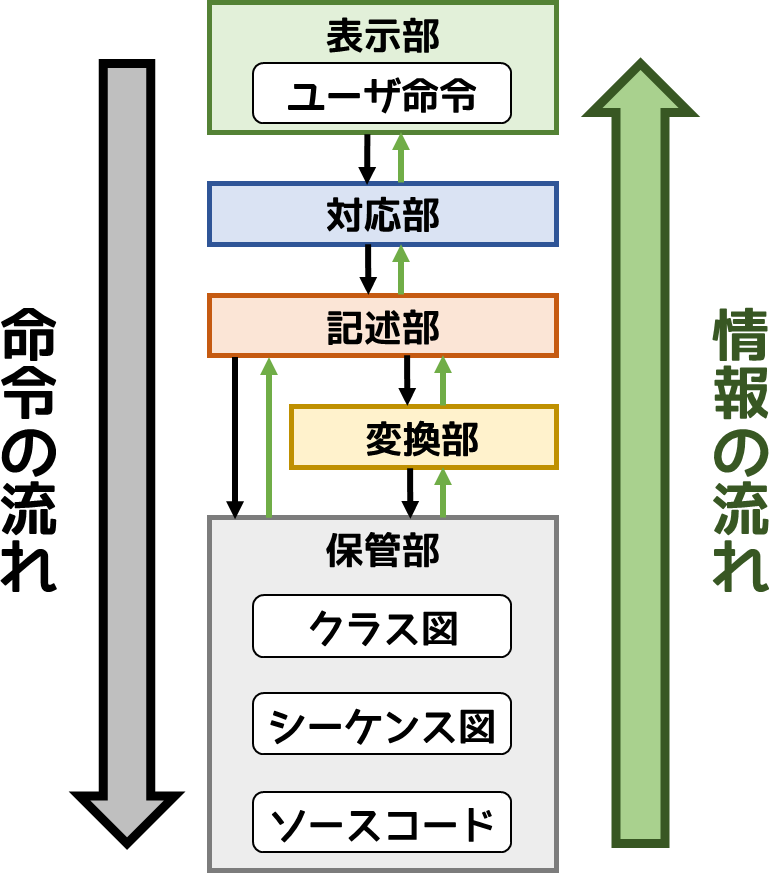
\includegraphics[keepaspectratio, width=160mm]{./figs/retussStructure.png}
	\caption{\tool{}の構造とデータ遷移}
	\label{fig:toolStructure2}
\end{center}
\end{figure}

% 適用例
\chapter{適用例}\label{cha:Indication}

% 考察
\chapter{考察}\label{cha:Evaluation}

% おわりに
\chapter{おわりに} \label{cha:Conclusion}

%%
% 謝辞
%
\acknowledgment{}

謝辞をかくよ


%%
% 参考文献
%
%%
% 参考文献
%
\bibliography{master} %hoge.bibから拡張子を外した名前
\bibliographystyle{junsrt} %参考文献出力スタイル

%%
% 付録
%
% \appendix{} % 付録は基本的に使わない

\end{document}
